%% LyX 2.3.6 created this file.  For more info, see http://www.lyx.org/.
%% Do not edit unless you really know what you are doing.
\documentclass[english]{article}
\usepackage[T1]{fontenc}
\usepackage[latin9]{inputenc}
\usepackage{float}
\usepackage{url}
\usepackage{amsmath}
\usepackage{graphicx}

\makeatletter

%%%%%%%%%%%%%%%%%%%%%%%%%%%%%% LyX specific LaTeX commands.
%% Because html converters don't know tabularnewline
\providecommand{\tabularnewline}{\\}
\floatstyle{ruled}
\newfloat{algorithm}{tbp}{loa}
\providecommand{\algorithmname}{Algorithm}
\floatname{algorithm}{\protect\algorithmname}

%%%%%%%%%%%%%%%%%%%%%%%%%%%%%% User specified LaTeX commands.

\newcommand{\argmin}{\mathop{\mathrm{arg\,min}}}

\makeatother

\usepackage{babel}
\begin{document}
\title{An improved multistart based method for global optimization problems}
\author{Ioannis G. Tsoulos\thanks{Corresponding author. Email: itsoulos@uoi.gr},
Alexandros Tzallas}
\date{Department of Informatics and Telecommunications, University of Ioannina,
Greece}
\maketitle
\begin{abstract}
There is a great need to discover the global optimum of multimodal
functions that arises from many scientifical and practical problems.
A base method used to solve this problem is the Multistart method.
The proposed method extends the traditional method by adding two major
features: the first one is a rejection mechanism to prevent the method
from spending time in unnecessary function evaluations and the second
is a stopping rule aimed to terminate the method when the global minimum
has been located with some certainty. The proposed method has been
evaluated on a series of global optimization functions from the relevant
literature and it is compared against some other optimization methods
and the experimental results are presented.
\end{abstract}
\textbf{Keywords}: Global optimization, stochastic methods, termination
rules.

\section{Introduction }

A novel method for the task of locating the global minimum of a continuous
and differentiable function $f:S\rightarrow R,S\subset R^{n}$ is
introduced here. The task of locating the global optimum can be formulated
as, determine 
\begin{equation}
x^{*}=\mbox{arg}\min_{x\in S}f(x)\label{eq:eq1}
\end{equation}
with $S$: 
\[
S=\left[a_{1},b_{1}\right]\otimes\left[a_{2},b_{2}\right]\otimes\ldots\left[a_{n},b_{n}\right]
\]
Methods that discover the global minimum can be used in many areas
such as: economics \cite{global_econ1,global_econ2}, physics \cite{global_physics1,global_physics2},
chemistry \cite{global_chemistry1,global_chemistry2}, medicine \cite{global_med1,global_med2}
etc. Global optimization methods usually are divided into two main
categories: deterministic and stochastic methods. The most common
methods of the first category are the so called Interval methods \cite{interval1,interval2},
where the set $S$ is divided iteratively in subregions and some subregions
that not contain the global solution are discarded using some pre
defined criteria. On the other hand, in the second category there
are Controlled Random Search methods \cite{crs1,crs2,crs3}, Simulated
Annealing methods \cite{simann_major,simann1,simann2}, Differential
Evolution methods \cite{diffe1,diffe2}, Particle Swarm Optimization
methods \cite{pso_major,pso1,pso2}, Ant Colony Optimization \cite{aco1,aco2},
Genetic algorithms \cite{ga1,ga2,ga3} etc. Also many hybrid methods
have been proposed such as combing the Simplex method and Inductive
search \cite{hybrid1}, methods that using PSO in conjuction with
other methods \cite{hybrid2,hybrid3}, etc. Recently many works have
been appeared that take advantage of the GPU processing units to implement
parallel global optimization methods \cite{gpu1,gpu2,gpu3}. 

This article introduces a novel method which is based on the multistart
method to discover the global minimum of continuous functions. The
method incorporates an efficient stopping rule as well as an asymptotic
criterion to prevent the algorithm from unnecessary local optimization
calls. The multistart method is one of the simplest global optimization
technique which starts a local optimization method from different
random samples and yields the lowest discovered minimum as the global
one. Due to its simplicity the method has been used in many problems
such as the TSP problem\textbf{ }\cite{multistart-tsp}, the vehicle
routing problem \cite{multistart-vehicle}, the facility location
problem \cite{multistart_fac}, the maximum clique problem \cite{multistart_clique},
the maximum fire risk insured capital problem \cite{multistart_fire},
aerodynamic shape problems \cite{multistart-aero} etc. During the
past year, the method multistart has been enhanced in the relevant
literature with methods that target to discover all the local minima
of a function \cite{tmlsl,Salhi,minfinder}, hybrid multistart techniques
\cite{mshybrid1,mshybrid2}, GRASP methods\cite{grasp}, new stopping
rules \cite{msstop1,msstop2,msstop3}, parallel techniques\cite{parallel-multistart,parallel-multistart2},
methods that utlize the modern GPU architectures to execute \cite{msgpu1,msgpu2},
methods that introduces sampling in the multistart method using Neural
Networks \cite{mssampling2} etc.

The rest of this article is organized as follows: in section \ref{sec:Method-description}
the proposed method is described in detail, in section \ref{sec:Experiments}
the experimental results are demonstrated and finally in section \ref{sec:Conclusions}
some conclusions and guidelines for future work are provided. 

\section{Method description \label{sec:Method-description}}

At every iteration of the proposed method a number of samples is taken
in the bounding box of the objective problem. Some of them are considered
as starting points for a local search procedure and the rest are discarded.
The method continues until the maximum number of iterations is reached
or an asymptotic termination rule, defined in subsection \ref{subsec:Stopping-rule}
is satisfied. The main steps of the proposed algorithm are outlined
in Algorithm \ref{alg:The-main-steps}. In the following subsection
the main parts of the proposed algorithm which are the discarding
procedure and the proposed stopping rule are described in detail.

\begin{algorithm}
\caption{The main steps of the proposed algorithm.\label{alg:The-main-steps}}

\begin{enumerate}
\item \textbf{Initialization Step}
\begin{enumerate}
\item \textbf{Set} $K$, the maximum number of allowed iterations.
\item \textbf{Set} $N$, the number points that will be samples at each
iteration.
\item \textbf{Set} $r_{C}=0$, the distance for the gradient check algorithm.
\item \textbf{Set} $X^{*}=\emptyset$, the set of local minima discovered
by the local search procedure.
\end{enumerate}
\item \textbf{Main Step\label{enu:Main-Step}}
\begin{enumerate}
\item \textbf{For} $i=1..N$ \textbf{do}
\begin{enumerate}
\item \textbf{Sample} randomly a point $x\in$S.
\item \textbf{Check} if $x$ is a valid starting point for the local search
procedure using the method gradientCheck(x) given in algorithm \ref{alg:The-procedure-gradientCheck(x).}.
\item \textbf{If} gradientCheck(x)=false \textbf{then}
\begin{enumerate}
\item \textbf{Start} a local search procedure $y=L(x)$
\item \textbf{Update} the distance $r_{C}$ using the equation \ref{eq:eq2}.
\item If $x\notin X^{*}$ then $X^{*}=X^{*}\cup x$
\end{enumerate}
\item \textbf{End if}
\end{enumerate}
\item \textbf{End For}
\end{enumerate}
\item \textbf{Termination Check Step. }Check the termination rule as described
in subsection \ref{subsec:Stopping-rule}.
\begin{enumerate}
\item \textbf{If }the termination rule holds \textbf{then} terminate
\item \textbf{else goto} \ref{enu:Main-Step}
\item \textbf{End if}
\end{enumerate}
\end{enumerate}
\end{algorithm}

\begin{algorithm}
\caption{The procedure gradientCheck(x), used to reject points from being start
points of the local search procedure.\label{alg:The-procedure-gradientCheck(x).}}

\textbf{boolean} gradientCheck(x)
\begin{enumerate}
\item \textbf{Set} $d=\min_{y\in X^{*}}\left\Vert y-x\right\Vert $
\item \textbf{Set} $z=\arg\min_{y\in X^{*}}\left\Vert y-x\right\Vert $
\item \textbf{If} $d<r_{C}$ AND $\left(x-z\right)^{T}\left(\nabla f(x)-\nabla f(z)\right)>0$
\textbf{then return} true
\item \textbf{else return} false
\end{enumerate}
\textbf{end} gradientCheck
\end{algorithm}


\subsection{Discarding procedure}

The discarding procedure has two major elements:
\begin{itemize}
\item The first is the typical distance that is calculated after every local
search and it is given by 
\begin{equation}
r_{C}=\frac{1}{M}\sum_{i=1}^{M}\left\Vert x_{i}-x_{iL}\right\Vert \label{eq:eq2}
\end{equation}
where the local search procedure $L(x)$ initiates from $x_{i}$ and
$x_{iL}$ is the outcome of $L\left(x_{i}\right)$. If a point $x$
is close enough to an already discovered local minima then it is highly
possible that the point belongs to the so called region of attraction
of the minima. The region of attraction of a local minimum $z$ is
defined as:
\begin{equation}
A\left(z\right)=\left\{ x:x\in S,\ L(x)=z\right\} 
\end{equation}
\item The second element is a gradient check performed between a candidate
starting point and an already discovered local minimum. The value
of the objective function $f(x)$ near to an already discovered local
minimum can be calculated using:
\begin{equation}
f(x)\simeq f(z)+\frac{1}{2}\left(x-z\right)^{T}B\left(x-z\right)\label{eq:eq4}
\end{equation}
where $B$ is the Hessian matrix at the minimum $z.$ By taking gradients
in both sides of Equation \ref{eq:eq4} we obtain:
\begin{equation}
\nabla f(x)\simeq B\left(x-z\right)\label{eq:eq5}
\end{equation}
Of course equation \ref{eq:eq5} holds for any other point $y$ near
to $z$ 
\begin{equation}
\nabla f(y)\simeq B\left(y-z\right)\label{eq:eq6}
\end{equation}
By subtracting the equation $\ref{eq:eq6}$ from \ref{eq:eq5} and
by multiplying with $\left(x-y\right)^{T}$ we have the following
equation:
\begin{equation}
\left(x-y\right)^{T}\left(\nabla f(x)-\nabla f(y)\right)\simeq\left(x-y\right)^{T}B\left(x-y\right)^{T}>0\label{eq:eq7}
\end{equation}
\end{itemize}
The distance $r_{C}$ is used with conjunction with equation \ref{eq:eq7}
to reject a point. The method rejects points from being start points
if they are close enough to some other located local minima and in
the same time equation \ref{eq:eq7} holds. A measure to identify
if a point is close enough to some other located local minima is the
distance $r_{C}$ calculated after every local minimization.

In order to measure the efficiency of the above rejection procedure
two tests were performed on two benchmark functions: Rastrigin and
Exp16. In these test the proportion of local search starts over total
number of samples were measured. The plot of this measurement for
20 iterations is plotted in Figures \ref{fig:Plot-for-Rastrigin}
and \ref{fig:Plot-for-exp16} respectively.

\begin{figure}
\caption{Plot for the proportion of local search starts over total number of
samples for the Rastrigin function for the first 20 iterations. \label{fig:Plot-for-Rastrigin}}

\begin{centering}
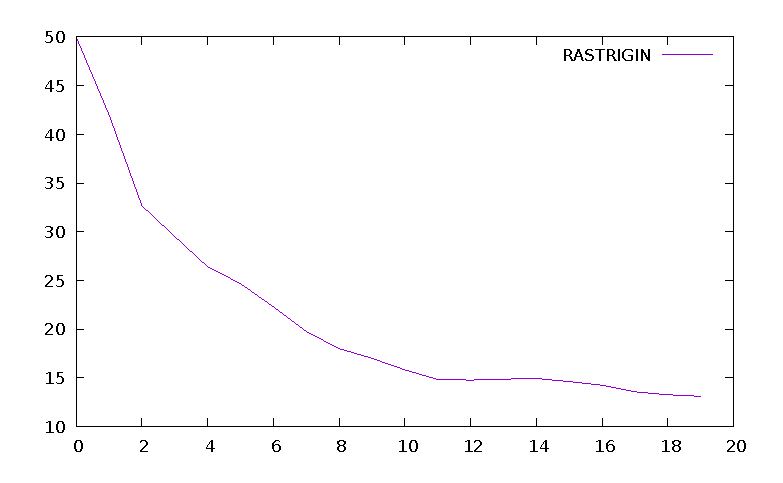
\includegraphics[scale=0.7]{rastrigin_start}
\par\end{centering}
\end{figure}
\begin{figure}
\caption{Plot for the proportion of local search starts over total number of
samples for the EXP16 function for the first 20 iterations.\label{fig:Plot-for-exp16}}

\begin{centering}
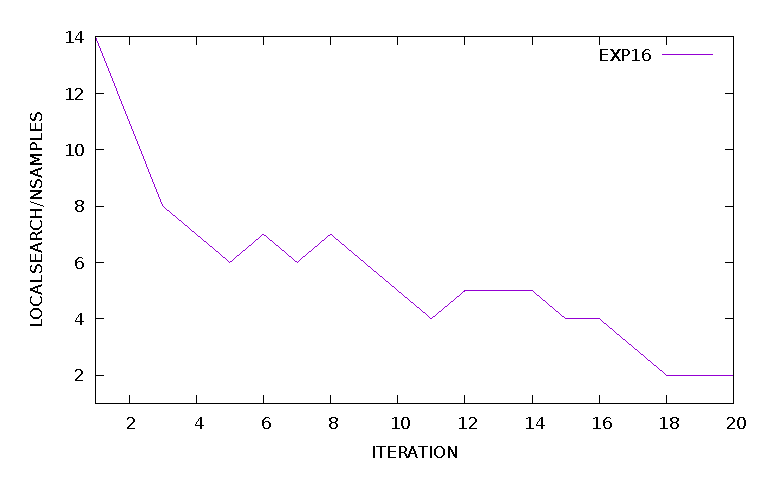
\includegraphics[scale=0.7]{exp16_start}
\par\end{centering}
\end{figure}


\subsection{Stopping rule\label{subsec:Stopping-rule}}

A common way to terminate a global optimization procedure is to use
the maximum number of allowed iterations, i.e. stop when $\mbox{iter}\ge K$.
Although, it is a simple criterion but is not an efficient one since,
if $K$ is tool small, then the algorithm will terminate without locating
the global optimum. Also, when $K$ is too high, the optimization
algorithm will spend computation time in unnecessary function calls.
The termination rule used here is derived from \cite{psotsoulos}:
denote with $\sigma^{(k)}$ the variance of $f\left(x^{*}\right)$,
where $k$ is the current iteration and $x^{*}$ is the so far located
global minimum. If the algorithm did not manage to locate new minimum
for a number of generations, then probably the algorithm has located
the global minimum and it should terminate. The termination rule stops
the algorithm when 

\begin{equation}
k\ge k_{\mbox{min}}\ \mbox{AND\ }\sigma^{(k)}\le\frac{\sigma^{\left(k_{\mbox{last}}\right)}}{2}\label{eq:termination_mine}
\end{equation}
where $k_{\mbox{last}}$ stands for iteration where a new minimum
was found. The value $k_{\mbox{min}}$ is a predefined minimum number
of iterations, in order to prevent the algorithm from premature termination.
In figure \ref{fig:Plot-of-variance} the values $\sigma^{(k)}$ denoted
as VARIANCE and the value $\frac{\sigma^{\left(k_{\mbox{last}}\right)}}{2}$
denoted as STOPAT are plotted. The objective function used is the
EXP8 function. The value of $k_{\mbox{min}}$ is set to 20 iterations
and the maximum number of iterations is 200. The algorithm terminates
successfully in 40 generation without spending unnecessary function
calls for about 160 generations. 

\begin{figure}
\caption{Plot of variance along with the stopping quantity for the problem
of Potential with 20 atoms.\label{fig:Plot-of-variance}}

\centering{}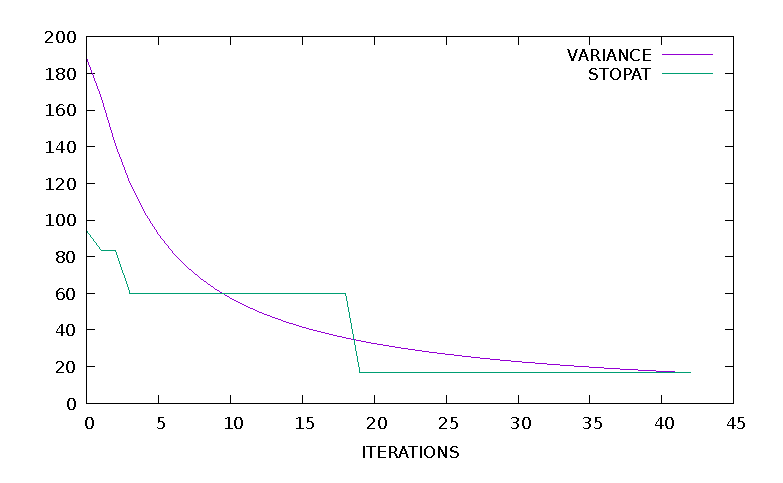
\includegraphics[scale=0.7]{termination_check}
\end{figure}


\subsection{Constrained optimization problems}

The proposed method can also be used to constrained optimization problems,
which general formulation is:
\begin{eqnarray}
\min_{x} & f(x) & \mbox{subject to}\nonumber \\
 & g_{i}(x)\le0 & \ i=1,\ldots,m\nonumber \\
 & h_{j}(x)=0 & \ j=1,\ldots,p\label{eq:eq1-1}
\end{eqnarray}
where $x_{i}\in\left[a_{i},b_{i}\right],\ i=1,\ldots,n$, which finds
application in many practical fields such as physics \cite{ConPhysics},
astronomy \cite{ConAstro}, chemistry \cite{ConChem}, biology \cite{ConBio}
etc. Many methods have been proposed to tackle this problem such as
Lagrange multiplier methods \cite{cons1}, Trust region methods \cite{cons2},
interval methods \cite{cons3}, methods based on differential evolution
\cite{cons4} etc. The constrained optimization problem can transformed
to a single function for the proposed method. The transformation is
performed in a way that when a solution is infeasible then the function
value is penalized according to the constraint violations. The steps
for the transformation are the following:\\

\begin{enumerate}
\item \textbf{Set} $v_{1}(x)=f(x)$
\item \textbf{Set} $v_{2}(x)=\sum_{i=1}^{p}h_{i}^{2}(x)$
\item \textbf{Calculate }for the inequality constraints $g_{i}(x),\ i=1,...,m$
the quantity 
\begin{equation}
v_{3}(x)=\sum_{i=1}^{m}G_{i}^{2}\left(g_{i}(x)\right)\label{eq:eq5-1}
\end{equation}
where the function $G(x)$ is defined as follows:
\begin{equation}
G(x)=\begin{cases}
0, & x\le0\\
x, & x>0
\end{cases}\label{eq:eq2-1}
\end{equation}
\item The transformed objective function for the proposed method is given
by:
\begin{equation}
v(x)=v_{1}(x)+\lambda v_{2}(x)+\lambda v_{3}(x)\label{eq:fitness}
\end{equation}
where $\lambda>0$.
\end{enumerate}

\section{Experiments\label{sec:Experiments}}

The proposed method was tested on a series of unconstrained and constrained
optimization functions that are listed in the Appendix. The local
search procedure in all experiments and methods was a BFGS variant
of Powell\cite{powell}. The method was tested against four methods
from the relevant literature:
\begin{enumerate}
\item Multistart method. This is simple method, who samples a series of
points each time (the same number as the proposed method) and performs
a local search procedure from every sample. In order to be the results
comparable against the proposed method the same stopping rule was
used also in the Multistart method. The code was implemented in ANSI
C++.
\item Multistart method with the repulsion sampling technique \cite{repulsion}
(title MREP). During the repulsion sampling, any produced sample is
repelled to a new location by the old starting points, in order to
avoid already visited regions of attraction.
\item Controlled Random Search denoted as CRS in the results. The implementation
used here is based on the algorithm of Price\cite{crs1} made in Ansi
C++. The method uses the suggested $N=25n$ from price value for the
initial number of samples in the set. Also, the implementation utilizes
the application of the Local search procedure after the termination
of the algorithm to enhance the located global optimum.
\item Simulated Annealing, denoted as SA in the results. The used software
here is the work of Corana\cite{corana}. 
\item Particle swarm optimization\cite{pso_major}, denoted as PSO in the
results. The implemented software here is coded in ANSI C++ and utilizes
the same stopping rule as in the proposed method. 
\end{enumerate}
The experimental results are reported in Table \ref{tab:Average-number-of}.
The number in the cells denotes average function calls for 30 runs
using with seed for the random generator each time. The fraction in
parentheses stands for the fraction of runs where the global optimum
was found. If this number is missing then the global minimum was discovered
in every independent run (100\% success). The parameters used in the
experiments are listed in Table \ref{tab:Parameter-values-for}. The
bold letters were used to demonstrate the method that achieved the
best average result. The proposed method seems to require less number
of function calls than the other methods and the PSO technique shown
to work well for small problems like BF1 or BRANIN but failed to work
on bigger problems such Potential20, a problem with dimension 60 and
thousands of local minima. On the other hand, the Simulated Annealing
managed to solve with success all the optimization problems, although
it requires more function calls than the proposed method and the same
holds for the simple Multistart method. Also, the Repulsion method
seems to overcome the simple Multistart but in the majority of cases
require significant more function calls than the proposed method.

In Table \ref{tab:Results-from-comparisons} the results from the
comparison of Multistart and the proposed method for the constrained
optimization test problems are listed. Again, the proposed method
has managed to handle the test problems using less number of function
evaluations than the Multistart method. The value of $\lambda=100$
was used for the conducted experiments. Again, the proposed method
overcomes the Multistart method to solve constrained optimization
problems. 

Also, in order to measure the efficiency of the proposed method for
as the dimension of the objective functions increases an additional
experiments was conducted: The function Exponential was used with
different values of the dimension $n$ from 2 to 20. The proposed
method is tested against Multistart and the results are plotted in
Figure \ref{fig:Average-number-of}. The average function calls required
by the proposed method are in the range {[}4000,6000{]} when the Multistart
requires 5 or 6 times more function calls. 

Additionally another experiment was conducted using the Exponential
function with $n=10$ with different values for the number of samples
$N$ and the results are plotted in Figure \ref{fig:Average-number-of-1}.
Again the Multistart requires much more function calls than the proposed
method and also the Multistart function calls tends to increase very
rapidly as compared to the calls of the proposed method.

To compare the proposed method with all the rest methods for different
function calls, the Wilcoxon signed-rank test was used. The results
obtained with this statistical test are shown in Figure \ref{fig:Box-plot-representation}.
The results indicate that the proposed method is superior than the
most of unconstrained optimization function (multistart, CSA and SA).
There was not, however, a significant difference between PSO and the
proposed method. 

\begin{table}
\caption{Average number of function calls for the proposed functions. \label{tab:Average-number-of}}

\begin{centering}
\begin{tabular}{|c|c|c|c|c|c|c|}
\hline 
PROBLEM & MULTISTART & MREP & CRS & SA & PSO & PROPOSED\tabularnewline
\hline 
\hline 
BF1 & 22533 & 5767 & 2218 & 3845 & \textbf{2494} & 2833\tabularnewline
\hline 
BF2 & 18809 & 4873 & 2207 & 3340 & 2641 & \textbf{2629}\tabularnewline
\hline 
BRANIN & 9735 & 4221 & 1744 & 4816 & \textbf{1636} & 1753\tabularnewline
\hline 
CM4 & 27037 & 15216 & 4746 & 9652 & 2988 & \textbf{2293}\tabularnewline
\hline 
CAMEL & 13688 & 4828 & 1882 & 4820 & \textbf{1639} & 1732\tabularnewline
\hline 
DIFFPOWER10 & 1194776 & 67129 & 78634 & 25918 & 15500(0.87) & \textbf{19572}\tabularnewline
\hline 
EASOM & 5372 & 3834 & 588 & 4807 & 866 & \textbf{199}\tabularnewline
\hline 
EXP8 & 12022 & 7226 & 13239 & 19233 & 3084 & \textbf{2830}\tabularnewline
\hline 
EXP32 & 18294 & 7600 & 93520 & 76842 & 5055 & \textbf{3265}\tabularnewline
\hline 
GKLS250 & 17333(0.77) & 3854 & 1633 & 4120 & \textbf{1459} & 2415\tabularnewline
\hline 
GKLS350 & 10104 & 5081 & 3329 & 7229 & 2259(0.97) & \textbf{243}\tabularnewline
\hline 
GRIEWANK2 & 13003 & 5031 & 2111 & 3830 & 2595(0.83) & \textbf{1786}\tabularnewline
\hline 
GRIEWANK10 & 53372 & 28289 & 32037 & 24118 & 8378(0.25) & \textbf{7184}\tabularnewline
\hline 
HANSEN & 15294 & 5268(0.97) & 3348 & 3323 & 4284 & \textbf{1510}\tabularnewline
\hline 
HARTMAN3 & 14815 & 5807 & 2898 & 7227 & \textbf{2448} & 11463\tabularnewline
\hline 
HARTMAN6 & 19459 & 7598 & 9276 & 14440 & 4645 & \textbf{3740}\tabularnewline
\hline 
POTENTIAL5 & 111631 & 29281 & 95027 & 36084 & \textbf{20100} & 49601\tabularnewline
\hline 
POTENTIAL10 & 208405 & \textbf{73080} & 193066 & 172166 & 19610(0.13) & 91094\tabularnewline
\hline 
POTENTIAL20 & 280575 & \textbf{135164} & 189591(0.53) & 244314 & 18466(0.03) & 170524(0.97)\tabularnewline
\hline 
RASTRIGIN & 16968 & 4706 & 1906 & 3343 & 2258 & \textbf{675}\tabularnewline
\hline 
SHEKEL5 & 19224 & 6456 & 6345 & 9635 & 4791 & \textbf{3465}\tabularnewline
\hline 
SHEKEL7 & 20985 & 7116 & 6528 & 9334 & 5722 & \textbf{2976}\tabularnewline
\hline 
SHEKEL10 & 20284 & 6968 & 6477 & 9998 & 5354 & \textbf{3566}\tabularnewline
\hline 
SINU8 & 21860 & 13183 & 16950 & 19241 & 5398 & \textbf{549}\tabularnewline
\hline 
SINU32 & 39905 & 92562 & 100887 & 13858 & 6887 & \textbf{1296}\tabularnewline
\hline 
TEST2n4 & 15938 & 9860 & 6754 & 9631 & 5219 & \textbf{2890}\tabularnewline
\hline 
TEST2n5 & 18085 & 11190 & 12717 & 12036 & 7672 & \textbf{3262}\tabularnewline
\hline 
TEST2n6 & 19879 & 13185 & 12822 & 14438 & 8039 & \textbf{3451}\tabularnewline
\hline 
TEST2n7 & 21432 & 14579 & 18620 & 16840 & 8220 & \textbf{4002}\tabularnewline
\hline 
TEST30n3 & 24450 & 13644 & 2768 & 9616 & \textbf{2456} & 10818\tabularnewline
\hline 
TEST30n4 & 26514 & 12004 & \textbf{3894} & 10617 & 4528 & 13320\tabularnewline
\hline 
\end{tabular}
\par\end{centering}
\end{table}
\begin{table}
\caption{Parameter values for the experiments. The parameters are hold for
Multistart, the Repulsion method and the proposed method. \label{tab:Parameter-values-for}}

\centering{}%
\begin{tabular}{|c|c|}
\hline 
PARAMETER & VALUE\tabularnewline
\hline 
\hline 
$K$ & 200\tabularnewline
\hline 
$N$ & 25\tabularnewline
\hline 
$k_{\mbox{min}}$ & 20\tabularnewline
\hline 
\end{tabular}
\end{table}
\begin{figure}
\caption{Average number of function calls for the function Exponential, as
the dimension of the function increases.\label{fig:Average-number-of}}

\centering{}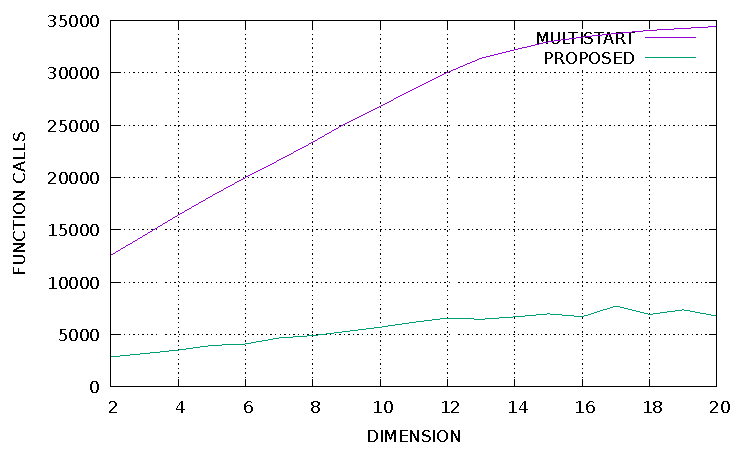
\includegraphics[scale=0.7]{expplot}
\end{figure}
\begin{figure}
\caption{Average number of function calls as the number of samples increases
for the function EXP10.\label{fig:Average-number-of-1}}

\begin{centering}
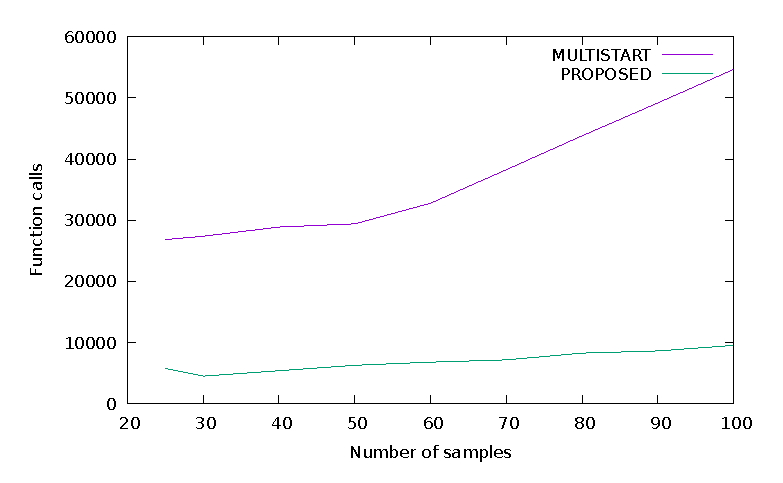
\includegraphics[scale=0.7]{plotsamples}
\par\end{centering}
\end{figure}
\begin{table}
\caption{Average function calls from comparisons of the proposed method and
Multistart for the constrained optimization problems.\label{tab:Results-from-comparisons}}

\centering{}%
\begin{tabular}{|c|c|c|}
\hline 
PROBLEM & MULTISTART & PROPOSED\tabularnewline
\hline 
\hline 
Levy & 17491 & 1301\tabularnewline
\hline 
Salkin & 48816 & 1010\tabularnewline
\hline 
Hess & 27775 & 9524\tabularnewline
\hline 
Chootinan1 & 293459 & 15035\tabularnewline
\hline 
G15 & 318162 & 63542\tabularnewline
\hline 
\end{tabular}
\end{table}
\begin{figure}

\caption{Box plot representation and Wilcoxon rank-sum test results of the
comparison between the multistart, CRS, SA, and PSO method and the
proposed method. A p-value of less than 0.05 (2-tailed) was used for
statistical significance and has been marked with bold. \label{fig:Box-plot-representation}}

\centering{}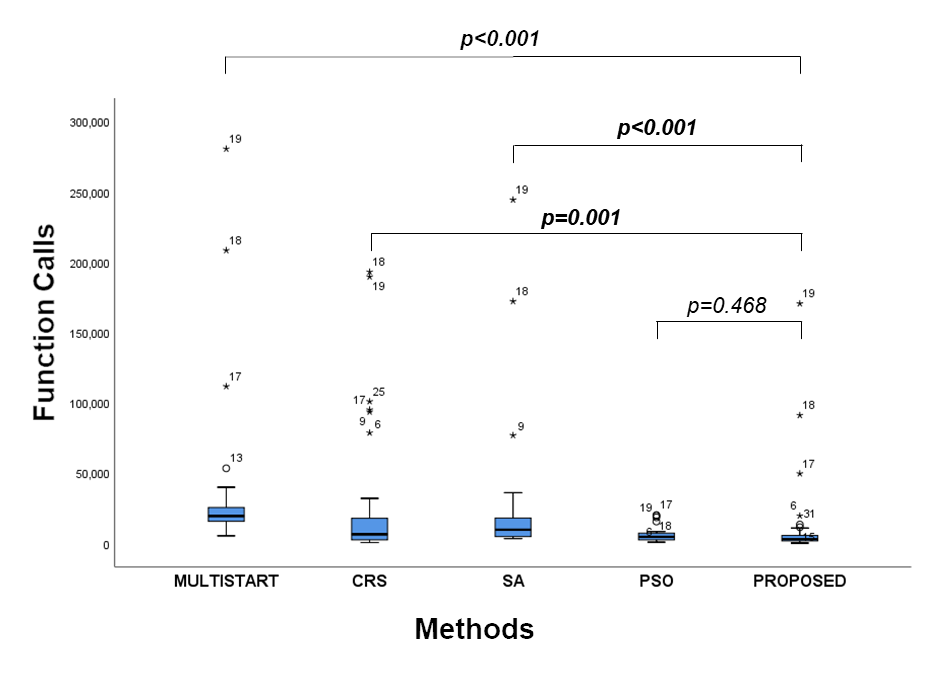
\includegraphics{methods_comparison}
\end{figure}


\section{Conclusions\label{sec:Conclusions}}

A novel multistart based method is described and tested here for global
optimization problems. The method utilizes an efficient discarding
procedure to prevent the method from unnecessary function calls and
an asymptotic stopping rule to stop the algorithm where there is a
good probability that the global optimum has been discovered. The
method was tested on a series of well known optimization problems
from the relevant literature and proved to be efficient and fast. 

\section*{Appendix - Test functions}

In order to measure the effectiveness of the proposed approach we
utilize several benchmark functions from the relevant literature \cite{Ali1,Floudas1}.

\subsection*{Unconstrained optimization functions}
\begin{itemize}
\item \textbf{Bf1} function. The function Bohachevsky 1 is given by the
equation
\end{itemize}
\[
f(x)=x_{1}^{2}+2x_{2}^{2}-\frac{3}{10}\cos\left(3\pi x_{1}\right)-\frac{4}{10}\cos\left(4\pi x_{2}\right)+\frac{7}{10}
\]
with $x\in[-100,100]^{2}$. The value of global minimum is 0.0.
\begin{itemize}
\item \textbf{Bf2} function. The function Bohachevsky 2 is given by the
equation 
\[
f(x)=x_{1}^{2}+2x_{2}^{2}-\frac{3}{10}\cos\left(3\pi x_{1}\right)\cos\left(4\pi x_{2}\right)+\frac{3}{10}
\]
with $x\in[-50,50]^{2}$. The value of the global minimum is 0.0.
\item \textbf{Branin} function. The function is defined by $f(x)=\left(x_{2}-\frac{5.1}{4\pi^{2}}x_{1}^{2}+\frac{5}{\pi}x_{1}-6\right)^{2}+10\left(1-\frac{1}{8\pi}\right)\cos(x_{1})+10$
with $-5\le x_{1}\le10,\ 0\le x_{2}\le15$. The value of global minimum
is 0.397887.with $x\in[-10,10]^{2}$. The value of global minimum
is -0.352386.
\item \textbf{CM} function. The Cosine Mixture function is given by the
equation 
\[
f(x)=\sum_{i=1}^{n}x_{i}^{2}-\frac{1}{10}\sum_{i=1}^{n}\cos\left(5\pi x_{i}\right)
\]
with $x\in[-1,1]^{n}$. The value of the global minimum is -0.4 and
in our experiments we have used $n=4$.
\item \textbf{Camel} function. The function is given by 
\[
f(x)=4x_{1}^{2}-2.1x_{1}^{4}+\frac{1}{3}x_{1}^{6}+x_{1}x_{2}-4x_{2}^{2}+4x_{2}^{4},\quad x\in[-5,5]^{2}
\]
The global minimum has the value of $f\left(x^{*}\right)=-1.0316$
\item \textbf{DiffPower} function. The Sum of Different Powers function
is defined 
\[
f(x)=\sum_{i=1}^{n}\left|x_{i}\right|^{i+1}
\]
and the global minimum is is $f\left(x^{*}\right)=0$. The value $n=10$
was used in the conducted experiments and the associated function
is denoted as Diffpower10.
\item \textbf{Easom} function. The function is given by the equation 
\[
f(x)=-\cos\left(x_{1}\right)\cos\left(x_{2}\right)\exp\left(\left(x_{2}-\pi\right)^{2}-\left(x_{1}-\pi\right)^{2}\right)
\]
with $x\in[-100,100]^{2}.$ The value of the global minimum is -1.0
\item \textbf{Exponential} function. The function is given by 
\[
f(x)=-\exp\left(-0.5\sum_{i=1}^{n}x_{i}^{2}\right),\quad-1\le x_{i}\le1
\]
The global minimum is located at $x^{*}=(0,0,...,0)$ with value $-1$.
In our experiments we used this function with $n=8,32$ and the corresponding
functions are denoted by the labels EXP8,EXP32.
\item \textbf{Griewank2} function. The function is given by
\[
f(x)=1+\frac{1}{200}\sum_{i=1}^{2}x_{i}^{2}-\prod_{i=1}^{2}\frac{\cos(x_{i})}{\sqrt{(i)}},\quad x\in[-100,100]^{2}
\]
The global minimum is located at the $x^{*}=(0,0,...,0)$ with value
0.
\item \textbf{Griewank10} function. The function is given by the equation
\[
f(x)=\sum_{i=1}^{n}\frac{x_{i}^{2}}{4000}-\prod_{i=1}^{n}\cos\left(\frac{x_{i}}{\sqrt{i}}\right)+1
\]
In our experiments we have used $n=10$ and the global minimum is
0.0 The function has several local minima in the specified range.
\item \textbf{Gkls} function. $f(x)=\mbox{Gkls}(x,n,w)$, is a function
with $w$ local minima, described in \cite{gkls} with $x\in[-1,1]^{n}$
and $n$ a positive integer between 2 and 100. The value of the global
minimum is -1 and in our experiments we have used $n=2,3$ and $w=50$.
The corresponding functions are denoted by the labels GKLS250 and
GKLS350. 
\item \textbf{Hansen} function. $f(x)=\sum_{i=1}^{5}i\cos\left[(i-1)x_{1}+i\right]\sum_{j=1}^{5}j\cos\left[(j+1)x_{2}+j\right]$,
$x\in[-10,10]^{2}$ . The global minimum of the function is -176.541793.
\item \textbf{Hartman 3} function. The function is given by
\[
f(x)=-\sum_{i=1}^{4}c_{i}\exp\left(-\sum_{j=1}^{3}a_{ij}\left(x_{j}-p_{ij}\right)^{2}\right)
\]
with $x\in[0,1]^{3}$ and $a=\left(\begin{array}{ccc}
3 & 10 & 30\\
0.1 & 10 & 35\\
3 & 10 & 30\\
0.1 & 10 & 35
\end{array}\right),\ c=\left(\begin{array}{c}
1\\
1.2\\
3\\
3.2
\end{array}\right)$ and
\[
p=\left(\begin{array}{ccc}
0.3689 & 0.117 & 0.2673\\
0.4699 & 0.4387 & 0.747\\
0.1091 & 0.8732 & 0.5547\\
0.03815 & 0.5743 & 0.8828
\end{array}\right)
\]
The value of global minimum is -3.862782.
\item \textbf{Hartman 6} function.
\[
f(x)=-\sum_{i=1}^{4}c_{i}\exp\left(-\sum_{j=1}^{6}a_{ij}\left(x_{j}-p_{ij}\right)^{2}\right)
\]
with $x\in[0,1]^{6}$ and $a=\left(\begin{array}{cccccc}
10 & 3 & 17 & 3.5 & 1.7 & 8\\
0.05 & 10 & 17 & 0.1 & 8 & 14\\
3 & 3.5 & 1.7 & 10 & 17 & 8\\
17 & 8 & 0.05 & 10 & 0.1 & 14
\end{array}\right),\ c=\left(\begin{array}{c}
1\\
1.2\\
3\\
3.2
\end{array}\right)$ and
\[
p=\left(\begin{array}{cccccc}
0.1312 & 0.1696 & 0.5569 & 0.0124 & 0.8283 & 0.5886\\
0.2329 & 0.4135 & 0.8307 & 0.3736 & 0.1004 & 0.9991\\
0.2348 & 0.1451 & 0.3522 & 0.2883 & 0.3047 & 0.6650\\
0.4047 & 0.8828 & 0.8732 & 0.5743 & 0.1091 & 0.0381
\end{array}\right)
\]
the value of global minimum is -3.322368.
\item \textbf{Potential} function. The molecular conformation corresponding
to the global minimum of the energy of N atoms interacting via the
Lennard-Jones potential\cite{Jones} is used as a test case here.
The function to be minimized is given by:
\begin{equation}
V_{LJ}(r)=4\epsilon\left[\left(\frac{\sigma}{r}\right)^{12}-\left(\frac{\sigma}{r}\right)^{6}\right]\label{eq:potential}
\end{equation}
In the current experiments three different cases were studied: $N=5,\ 10,\ 20$
\item \textbf{Rastrigin} function. The function is given by 
\[
f(x)=x_{1}^{2}+x_{2}^{2}-\cos(18x_{1})-\cos(18x_{2}),\quad x\in[-1,1]^{2}
\]
The global minimum is located at $x^{*}=(0,0)$ with value -2.0.
\item \textbf{Shekel 7} function.
\end{itemize}
\[
f(x)=-\sum_{i=1}^{7}\frac{1}{(x-a_{i})(x-a_{i})^{T}+c_{i}}
\]

with $x\in[0,10]^{4}$ and $a=\left(\begin{array}{cccc}
4 & 4 & 4 & 4\\
1 & 1 & 1 & 1\\
8 & 8 & 8 & 8\\
6 & 6 & 6 & 6\\
3 & 7 & 3 & 7\\
2 & 9 & 2 & 9\\
5 & 3 & 5 & 3
\end{array}\right),\ c=\left(\begin{array}{c}
0.1\\
0.2\\
0.2\\
0.4\\
0.4\\
0.6\\
0.3
\end{array}\right)$. The value of global minimum is -10.342378.
\begin{itemize}
\item \textbf{Shekel 5 }function.
\end{itemize}
\[
f(x)=-\sum_{i=1}^{5}\frac{1}{(x-a_{i})(x-a_{i})^{T}+c_{i}}
\]
 

with $x\in[0,10]^{4}$ and $a=\left(\begin{array}{cccc}
4 & 4 & 4 & 4\\
1 & 1 & 1 & 1\\
8 & 8 & 8 & 8\\
6 & 6 & 6 & 6\\
3 & 7 & 3 & 7
\end{array}\right),\ c=\left(\begin{array}{c}
0.1\\
0.2\\
0.2\\
0.4\\
0.4
\end{array}\right)$. The value of global minimum is -10.107749.
\begin{itemize}
\item \textbf{Shekel 10} function.
\end{itemize}
\[
f(x)=-\sum_{i=1}^{10}\frac{1}{(x-a_{i})(x-a_{i})^{T}+c_{i}}
\]
 

with $x\in[0,10]^{4}$ and $a=\left(\begin{array}{cccc}
4 & 4 & 4 & 4\\
1 & 1 & 1 & 1\\
8 & 8 & 8 & 8\\
6 & 6 & 6 & 6\\
3 & 7 & 3 & 7\\
2 & 9 & 2 & 9\\
5 & 5 & 3 & 3\\
8 & 1 & 8 & 1\\
6 & 2 & 6 & 2\\
7 & 3.6 & 7 & 3.6
\end{array}\right),\ c=\left(\begin{array}{c}
0.1\\
0.2\\
0.2\\
0.4\\
0.4\\
0.6\\
0.3\\
0.7\\
0.5\\
0.6
\end{array}\right)$. The value of global minimum is -10.536410.
\begin{itemize}
\item \textbf{Sinusoidal} function. The function is given by 
\[
f(x)=-\left(2.5\prod_{i=1}^{n}\sin\left(x_{i}-z\right)+\prod_{i=1}^{n}\sin\left(5\left(x_{i}-z\right)\right)\right),\quad0\le x_{i}\le\pi.
\]
The global minimum is located at $x^{*}=(2.09435,2.09435,...,2.09435)$
with $f\left(x^{*}\right)=-3.5$. In our experiments we used $n=8,32$
and $z=\frac{\pi}{6}$ and the corresponding functions are denoted
by the labels SINU8 and SINU32 respectively.
\item \textbf{Test2N} function. This function is given by the equation 
\[
f(x)=\frac{1}{2}\sum_{i=1}^{n}x_{i}^{4}-16x_{i}^{2}+5x_{i},\quad x_{i}\in[-5,5].
\]
The function has $2^{n}$ in the specified range and in our experiments
we used $n=4,5,6,7$. The corresponding values of global minimum is
-156.664663 for $n=4$, -195.830829 for $n=5$, -234.996994 for $n=6$
and -274.163160 for $n=7$.
\item Test30N function. This function is given by 
\[
f(x)=\frac{1}{10}\sin^{2}\left(3\pi x_{1}\right)\sum_{i=2}^{n-1}\left(\left(x_{i}-1\right)^{2}\left(1+\sin^{2}\left(3\pi x_{i+1}\right)\right)\right)+\left(x_{n}-1\right)^{2}\left(1+\sin^{2}\left(2\pi x_{n}\right)\right)
\]
with $x\in[-10,10]$. The function has $30^{n}$ local minima in the
specified range and we used $n=3,4$ in our experiments. The value
of global minimum for this function is 0.0
\end{itemize}

\subsection*{Constrained optimization test fuctions}

The following functions were used from the relevant literature.
\begin{itemize}
\item \textbf{Levy} function. This problem is described in \cite{Levy}
and it is given by: 
\[
\min_{x}f(x)=-x_{1}-x_{2}
\]
with $x\in[0,1]^{2}$, subject to 
\[
g_{1}(x)=\left\lfloor \left(x_{1}-1\right)^{2}+\left(x_{2}-1\right)\right\rfloor \left(\frac{1}{2a^{2}}-\frac{1}{2b^{2}}\right)+\left(x_{1}-1\right)\left(x_{2}-1\right)\left(\frac{1}{a^{2}}-\frac{1}{b^{2}}\right)-1\ge0
\]
with $a=2,\ b=0.25$. The value of global minimum is $f_{\mbox{min}}=-1.8729$.
\item \textbf{Salkin} function. This problem is described in \cite{Salkin}
and it is given by: 
\[
\max_{x}f(x)=3x_{1}+x_{2}+2x_{3}+x_{4}-x_{5}
\]
with $1\le x_{1}\le4,\ 80\le x_{2}\le88,\ 30\le x_{3}\le35,\ 145\le x_{4}\le150,\ 0\le x_{5}\le2$
subject to 
\begin{eqnarray*}
g_{1}(x) & = & 25x_{1}-40x_{2}+16x_{3}+21x_{4}+x5\le300\\
g_{2}(x) & = & x_{1}+20x_{2}-50x_{3}+x_{4}-x_{5}\le200\\
g_{3}(x) & = & 60x_{1}+x_{2}-x_{3}+2x_{4}+x_{5}\le600\\
g_{4}(x) & = & -7x_{1}+4x_{2}+15x_{3}-x_{4}+65x_{5}\le700
\end{eqnarray*}
This global maximum is $f_{\mbox{max}}=320$.
\item \textbf{Hess} function. This problem is described in \cite{Hess}
and it is given by:
\[
\max_{x}f(x)=25\left(x_{1}-2\right)^{2}+\left(x_{2}-2\right)^{2}+\left(x_{3}-1\right)^{2}+\left(x_{4}-4\right)^{2}+\left(x_{5}-1\right)^{2}+\left(x_{6}-4\right)^{2}
\]
with $0\le x_{1}\le5,\ 0\le x_{2}\le1,\ 1\le x_{3}\le5,\ 0\le x_{4}\le6,\ 0\le x_{5}\le5,\ 0\le x_{6}\le10$
subject to:
\begin{eqnarray*}
g_{1}(x) & = & x_{1}+x_{2}-2\ge0\\
g_{2}(x) & = & -x_{1}+x_{2}+6\ge0\\
g_{3}(x) & = & x_{1}-x_{2}+2\ge0\\
g_{4}(x) & = & -x_{1}+3x_{2}+2\ge0\\
g_{5}(x) & = & \left(x_{3}-3\right)^{2}+x_{4}-4\ge0\\
g_{6}(x) & = & \left(x_{5}-3\right)^{2}+x_{6}-4\ge0
\end{eqnarray*}
The value of global maximum is $f_{\mbox{max}}=310.$
\item \textbf{Chootinan1} function. This problem is described in \cite{choot}
and it is given by:
\[
\min_{x}f(x)=5\sum_{i=1}^{4}x_{i}-5\sum_{i=1}^{4}x_{i}^{2}-\sum_{i=1}^{13}x_{i}
\]
with $0\le x_{i}\le1$ for $i=1,..,9,13$, $0\le x_{i}\le100$ for
$i=10,11,12$ with the following constraints:
\begin{eqnarray*}
g_{1}(x) & = & 10-\left(2x_{1}+2x_{2}+x_{10}+x_{11}\right)\ge0\\
g_{2}(x) & = & 10-\left(2x_{1}+2x_{3}+x_{10}+x_{12}\right)\ge0\\
g_{3}(x) & = & 10-\left(2x_{2}+2x_{3}+x_{11}+x_{12}\right)\ge0\\
g_{4}(x) & = & 8x_{1}-x_{10}\ge0\\
g_{5}(x) & = & 8x_{2}-x_{11}\ge0\\
g_{6}(x) & = & 8x_{3}-x_{12}\ge0\\
g_{7}(x) & = & 2x_{4}+x_{5}-x_{10}\ge0\\
g_{8}(x) & = & 2x_{6}+x_{7}-x_{11}\ge0\\
g_{9}(x) & = & 2x_{8}+x_{9}-x_{12}\ge0
\end{eqnarray*}
The value of global minimum is $f_{\mbox{min}}=-15.0$.
\item \textbf{G15} function. This problem is described in \cite{G15} and
it is given by:
\[
\min_{x}f(x)=1000-x_{1}^{2}-2x_{2}^{2}-x_{3}^{2}-x_{1}x_{2}-x_{1}x_{3}
\]
with $x\in[0,10]^{3}$ subject to the following constraints:
\begin{eqnarray*}
h_{1}(x) & = & x_{1}^{2}+x_{2}^{2}+x_{3}^{2}-25=0\\
h_{2}(x) & = & 8x_{1}+14x_{2}+7x_{3}-56=0
\end{eqnarray*}
The value of the global minimum is $f_{\mbox{min}}=961.7150$
\end{itemize}

\subsection*{Compliance with Ethical Standards }

All authors declare that they have no has no conict of interest. 

\subsection*{Acknowledgments}

The experiments of this research work was performed at the high performance
computing system established at Knowledge and Intelligent Computing
Lab-oratory, Dept of Informatics and Telecommunications, University
of Ioannina, acquired with the project \textquotedbl Educational
Laboratory equipment of TEI of Epirus\textquotedbl{} with MIS 5007094
funded by the Operational Programme \textquotedbl Epirus\textquotedbl{}
2014-2020, by ERDF and national finds.
\begin{thebibliography}{10}
\bibitem{global_econ1}Zwe-Lee Gaing, Particle swarm optimization
to solving the economic dispatch considering the generator constraints,
IEEE Transactions on \textbf{18} Power Systems, pp. 1187-1195, 2003.

\bibitem{global_econ2}C. D. Maranas, I. P. Androulakis, C. A. Floudas,
A. J. Berger, J. M. Mulvey, Solving long-term financial planning problems
via global optimization, Journal of Economic Dynamics and Control
\textbf{21}, pp. 1405-1425, 1997.

\bibitem{global_physics1}Q. Duan, S. Sorooshian, V. Gupta, Effective
and efficient global optimization for conceptual rainfall-runoff models,
Water Resources Research \textbf{28}, pp. 1015-1031 , 1992.

\bibitem{global_physics2}P. Charbonneau, Genetic Algorithms in Astronomy
and Astrophysics, Astrophysical Journal Supplement \textbf{101}, p.
309, 1995

\bibitem{global_chemistry1}A. Liwo, J. Lee, D.R. Ripoll, J. Pillardy,
H. A. Scheraga, Protein structure prediction by global optimization
of a potential energy function, Biophysics \textbf{96}, pp. 5482-5485,
1999.

\bibitem{global_chemistry2}P.M. Pardalos, D. Shalloway, G. Xue, Optimization
methods for computing global minima of nonconvex potential energy
functions, Journal of Global Optimization \textbf{4}, pp. 117-133,
1994.

\bibitem{global_med1}Eva K. Lee, Large-Scale Optimization-Based Classification
Models in Medicine and Biology, Annals of Biomedical Engineering \textbf{35},
pp 1095-1109, 2007.

\bibitem{global_med2}Y. Cherruault, Global optimization in biology
and medicine, Mathematical and Computer Modelling \textbf{20}, pp.
119-132, 1994.

\bibitem{interval1}M.A. Wolfe, Interval methods for global optimization,
Applied Mathematics and Computation \textbf{75}, pp. 179-206, 1996.

\bibitem{interval2}T. Csendes and D. Ratz, Subdivision Direction
Selection in Interval Methods for Global Optimization, SIAM J. Numer.
Anal. \textbf{34}, pp. 922--938, 1997. 

\bibitem{crs1}W. L. Price, Global optimization by controlled random
search, Journal of Optimization Theory and Applications \textbf{40},
pp. 333-348, 1983.

\bibitem{crs2}Ivan K\v{r}iv�, Josef Tvrd�k, The controlled random
search algorithm in optimizing regression models, Computational Statistics
\& Data Analysis \textbf{20}, pp. 229-234, 1995.

\bibitem{crs3}M.M. Ali, A. T�rn, and S. Viitanen, A Numerical Comparison
of Some Modified Controlled Random Search Algorithms, Journal of Global
Optimization \textbf{11},pp. 377--385,1997.

\bibitem{simann_major}S. Kirkpatrick, CD Gelatt, , MP Vecchi, Optimization
by simulated annealing, Science \textbf{220}, pp. 671-680, 1983.

\bibitem{simann1}L. Ingber, Very fast simulated re-annealing, Mathematical
and Computer Modelling \textbf{12}, pp. 967-973, 1989.

\bibitem{simann2}R.W. Eglese, Simulated annealing: A tool for operational
research, Simulated annealing: A tool for operational research \textbf{46},
pp. 271-281, 1990.

\bibitem{diffe1}R. Storn, K. Price, Differential Evolution - A Simple
and Efficient Heuristic for Global Optimization over Continuous Spaces,
Journal of Global Optimization \textbf{11}, pp. 341-359, 1997.

\bibitem{diffe2}J. Liu, J. Lampinen, A Fuzzy Adaptive Differential
Evolution Algorithm. Soft Comput \textbf{9}, pp.448--462, 2005.

\bibitem{pso_major}J. Kennedy and R. Eberhart, \textquotedbl Particle
swarm optimization,\textquotedbl{} Proceedings of ICNN'95 - International
Conference on Neural Networks, 1995, pp. 1942-1948 vol.4, doi: 10.1109/ICNN.1995.488968.

\bibitem{pso1}Riccardo Poli, James Kennedy kennedy, Tim Blackwell,
Particle swarm optimization An Overview, Swarm Intelligence \textbf{1},
pp 33-57, 2007. 

\bibitem{pso2}Ioan Cristian Trelea, The particle swarm optimization
algorithm: convergence analysis and parameter selection, Information
Processing Letters \textbf{85}, pp. 317-325, 2003.

\bibitem{aco1}M. Dorigo, M. Birattari and T. Stutzle, Ant colony
optimization, IEEE Computational Intelligence Magazine \textbf{1},
pp. 28-39, 2006.

\bibitem{aco2}K. Socha, M. Dorigo, Ant colony optimization for continuous
domains, European Journal of Operational Research 185, pp. 1155-1173,
2008.

\bibitem{ga1}D. Goldberg, Genetic Algorithms in Search, Optimization
and Machine Learning, Addison-Wesley Publishing Company, Reading,
Massachussets, 1989.

\bibitem{ga2}Z. Michaelewicz, Genetic Algorithms + Data Structures
= Evolution Programs. Springer - Verlag, Berlin, 1996.

\bibitem{ga3}S.A. Grady, M.Y. Hussaini, M.M. Abdullah, Placement
of wind turbines using genetic algorithms, Renewable Energy \textbf{30},
pp. 259-270, 2005.

\bibitem{hybrid1}Offord C., Bajzer �. (2001) A Hybrid Global Optimization
Algorithm Involving Simplex and Inductive Search. In: Alexandrov V.N.,
Dongarra J.J., Juliano B.A., Renner R.S., Tan C.J.K. (eds) Computational
Science - ICCS 2001. ICCS 2001. Lecture Notes in Computer Science,
vol 2074. Springer, Berlin, Heidelberg. https://doi.org/10.1007/3-540-45718-6\_73

\bibitem{hybrid2}M. Pant, R. Thangaraj, C. Grosan and A. Abraham,
\textquotedbl Hybrid Differential Evolution - Particle Swarm Optimization
Algorithm for Solving Global Optimization Problems,\textquotedbl{}
2008 Third International Conference on Digital Information Management,
2008, pp. 18-24, doi: 10.1109/ICDIM.2008.4746766.

\bibitem{hybrid3}Niu B., Li L. (2008) A Novel PSO-DE-Based Hybrid
Algorithm for Global Optimization. In: Huang DS., Wunsch D.C., Levine
D.S., Jo KH. (eds) Advanced Intelligent Computing Theories and Applications.
With Aspects of Artificial Intelligence. ICIC 2008. Lecture Notes
in Computer Science, vol 5227. Springer, Berlin, Heidelberg. https://doi.org/10.1007/978-3-540-85984-0\_20

\bibitem{gpu1}Y. Zhou and Y. Tan, \textquotedbl GPU-based parallel
particle swarm optimization,\textquotedbl{} 2009 IEEE Congress on
Evolutionary Computation, 2009, pp. 1493-1500, doi: 10.1109/CEC.2009.4983119.

\bibitem{gpu2}L. Dawson and I. Stewart, \textquotedbl Improving
Ant Colony Optimization performance on the GPU using CUDA,\textquotedbl{}
2013 IEEE Congress on Evolutionary Computation, 2013, pp. 1901-1908,
doi: 10.1109/CEC.2013.6557791.

\bibitem{gpu3}Barkalov, K., Gergel, V. Parallel global optimization
on GPU. J Glob Optim 66, 3--20 (2016). https://doi.org/10.1007/s10898-016-0411-y

\bibitem{multistart-tsp}Li W., A Parallel Multi-start Search Algorithm
for Dynamic Traveling Salesman Problem. In: Pardalos P.M., Rebennack
S. (eds) Experimental Algorithms. SEA 2011. Lecture Notes in Computer
Science, vol 6630. Springer, Berlin, Heidelberg, 2011.

\bibitem{multistart-vehicle}Olli Br�ysy, Geir Hasle, Wout Dullaert,
A multi-start local search algorithm for the vehicle routing problem
with time windows, European Journal of Operational Research \textbf{159},
pp. 586-605, 2004.

\bibitem{multistart_fac}Mauricio G.C. Resende, Renato F. Werneck,A
hybrid multistart heuristic for the uncapacitated facility location
problem, European Journal of Operational Research \textbf{174}, pp.
54-68, 2006.

\bibitem{multistart_clique}E. Marchiori, Genetic, Iterated and Multistart
Local Search for the Maximum Clique Problem. In: Cagnoni S., Gottlieb
J., Hart E., Middendorf M., Raidl G.R. (eds) Applications of Evolutionary
Computing. EvoWorkshops 2002. Lecture Notes in Computer Science, vol
2279. Springer, Berlin, Heidelberg. 

\bibitem{multistart_fire}Gomes M.I., Afonso L.B., Chibeles-Martins
N., Fradinho J.M. (2018) Multi-start Local Search Procedure for the
Maximum Fire Risk Insured Capital Problem. In: Lee J., Rinaldi G.,
Mahjoub A. (eds) Combinatorial Optimization. ISCO 2018. Lecture Notes
in Computer Science, vol 10856. Springer, Cham. https://doi.org/10.1007/978-3-319-96151-4\_19

\bibitem{multistart-aero}Streuber, Gregg M. and Zingg, David. W.,
Evaluating the Risk of Local Optima in Aerodynamic Shape Optimization,
AIAA Journal 59, pp. 75-87, 2012.

\bibitem{bfgs}Ya-Xiang Yuan, A Modified BFGS Algorithm for Unconstrained
Optimization, IMA Journal of Numerical Analysis \textbf{11}, pp. 325--332,
1991.

\bibitem{tmlsl}M.M. Ali, C. Storey, Topographical multilevel single
linkage, J. Global Optimization 5 (1994) 349--358

\bibitem{Salhi}S. Salhi, N.M. Queen, A hybrid algorithm for identifying
global and local minima when optimizing functions with many minima,
European J. Oper. Res. 155(2004) 51--67.

\bibitem{minfinder}I. G. Tsoulos and I. E. Lagaris, MinFinder: Locating
all the local minima of a function, Computer Physics Communications
\textbf{174}, pp. 166-179, 2006. 

\bibitem{mshybrid1}M. Perez, F. Almeida and J. M. Moreno-Vega, \textquotedbl Genetic
algorithm with multistart search for the p-Hub median problem,\textquotedbl{}
Proceedings. 24th EUROMICRO Conference (Cat. No.98EX204), Vasteras,
Sweden, 1998, pp. 702-707 vol.2.

\bibitem{mshybrid2}H. C. B. d. Oliveira, G. C. Vasconcelos and G.
B. Alvarenga, \textquotedbl A Multi-Start Simulated Annealing Algorithm
for the Vehicle Routing Problem with Time Windows,\textquotedbl{}
2006 Ninth Brazilian Symposium on Neural Networks (SBRN'06), Ribeirao
Preto, Brazil, 2006, pp. 137-142.

\bibitem{grasp}Festa P., Resende M.G.C. (2009) Hybrid GRASP Heuristics.
In: Abraham A., Hassanien AE., Siarry P., Engelbrecht A. (eds) Foundations
of Computational Intelligence Volume 3. Studies in Computational Intelligence,
vol 203. Springer, Berlin, Heidelberg. 

\bibitem{msstop1}B. Betro`, F. Schoen, Optimal and sub-optimal stopping
rules for the multistart algorithm in global optimization, Math. Program.
\textbf{57}, pp. 445--458, 1992.

\bibitem{msstop2}W.E. Hart, Sequential stopping rules for random
optimization methods with applications to multistart local search,
Siam J. Optim. \textbf{9}, pp. 270--290, 1998.

\bibitem{msstop3}I.E. Lagaris and I.G. Tsoulos, Stopping Rules for
Box-Constrained Stochastic Global Optimization, Applied Mathematics
and Computation \textbf{197}, pp. 622-632, 2008.

\bibitem{parallel-multistart}J. Larson and S.M. Wild, Asynchronously
parallel optimization solver for finding multiple minima, Mathematical
Programming Computation \textbf{10}, pp. 303-332, 2018.

\bibitem{parallel-multistart2}H.P.J. Bolton, J.F. Schutte, A.A. Groenwold,
Multiple Parallel Local Searches in Global Optimization. In: Dongarra
J., Kacsuk P., Podhorszki N. (eds) Recent Advances in Parallel Virtual
Machine and Message Passing Interface. EuroPVM/MPI 2000. Lecture Notes
in Computer Science, vol 1908. Springer, Berlin, Heidelberg, 2000.

\bibitem{msgpu1}R. Kamil, S. Reiji, An Efficient GPU Implementation
of a Multi-Start TSP Solver for Large Problem Instances, Proceedings
of the 14th Annual Conference Companion on Genetic and Evolutionary
Computation, pp. 1441-1442, 2012.

\bibitem{msgpu2}Van Luong T., Melab N., Talbi EG. (2011) GPU-Based
Multi-start Local Search Algorithms. In: Coello C.A.C. (eds) Learning
and Intelligent Optimization. LION 2011. Lecture Notes in Computer
Science, vol 6683. Springer, Berlin, Heidelberg. https://doi.org/10.1007/978-3-642-25566-3\_24

\bibitem{mssampling2}I.G. Tsoulos, E. Karvounis, A. Tzallas, A Novel
Sampling Technique for Multistart-Based Methods, SN Computer Science
2, pp.7, 2021.

\bibitem{psotsoulos}Ioannis G. Tsoulos, Modifications of real code
genetic algorithm for global optimization, Applied Mathematics and
Computation \textbf{203}, pp. 598-607, 2008.

\bibitem{powell}M.J.D Powell, A Tolerant Algorithm for Linearly Constrained
Optimization Calculations, Mathematical Programming \textbf{45}, pp.
547-566, 1989. 

\bibitem{corana}{[}3{]} A. Corana, M. Marchesi, C. Martini, S. Ridella,
Minimizing multimodal functions of continuous variables with the \textquotedblleft Simulated
Annealing\textquotedblright{} algorithm, ACM Trans. Math. Software
13 (1987) 262--280. 

\bibitem{repulsion}A.E. Sepulveda, L. Epstein, The repulsion algorithm
a new multistart method for global optimization, Structural Optimization
\textbf{11}, pp. 145-152, 1996 

\bibitem{Ali1}M. Montaz Ali, Charoenchai Khompatraporn, Zelda B.
Zabinsky, A Numerical Evaluation of Several Stochastic Algorithms
on Selected Continuous Global Optimization Test Problems, Journal
of Global Optimization \textbf{31}, pp 635-672, 2005. 

\bibitem{Floudas1}C.A. Floudas, P.M. Pardalos, C. Adjiman, W. Esposoto,
Z. G$\ddot{\mbox{u}}$m$\ddot{\mbox{u}}$s, S. Harding, J. Klepeis,
C. Meyer, C. Schweiger, Handbook of Test Problems in Local and Global
Optimization, Kluwer Academic Publishers, Dordrecht, 1999.

\bibitem{gkls}M. Gaviano, D.E. Ksasov, D. Lera, Y.D. Sergeyev, Software
for generation of classes of test functions with known local and global
minima for global optimization, ACM Trans. Math. Softw. \textbf{29},
pp. 469-480, 2003.

\bibitem{Jones}J.E. Lennard-Jones, On the Determination of Molecular
Fields, Proc. R. Soc. Lond. A \textbf{ 106}, pp. 463--477, 1924.

\bibitem{ConPhysics}O.A. Sauer, D.M. Shepard, T.R. Mackie, Application
of constrained optimization to radiotherapy planning, Medical Physics
\textbf{26}, pp. 2359-2366, 1999.

\bibitem{ConAstro}F.P. Seelos, R.E. Arvidson, Bounded variable least
squares - application of a constrained optimization algorithm to the
analysis of TES Emissivity Spectra, in: 34th Annual Lunar and Planetary
Science Conference, March 17-21, 2003, League City, Texas, abstract
no.1817.

\bibitem{ConChem}M.J. Field, Constrained optimization of ab initio
and semiempirical Hartree-Fock wave functions using direct minimization
or simulated annealing , Journal of physical chemistry \textbf{95},
pp. 5104-5108, 1991.

\bibitem{ConBio}G.A. Williams, J.M. Dugan, R.B. Altman, Constrained
global optimization for estimating molecular structure from atomic
distances, Journal of Computational Biology \textbf{8}, pp. 523-547,
2001.

\bibitem{cons1}P.E. Gill, W. Murray, The computation of Lagrange-multiplier
estimates for constrained minimization, Mathematical Programming \textbf{17},
pp. 32-60, 1979.

\bibitem{cons2}M.J.D. Powell, Y. Yuan, A trust region algorithm for
equality constrained optimization, Mathematical Programming \textbf{49},
pp. 189-211, 2005.

\bibitem{cons3}K. Ichida, Constrained optimization using interval
analysis, Computers and Industrial Engineering \textbf{31}, pp. 933-937,
1996.

\bibitem{cons4}R.L. Becerra, C.A.C. Coello, Cultured differential
evolution for constrained optimization, Computer Methods in Applied
Mechanics and Engineering \textbf{195}, pp. 4303-4322, 2006.

\bibitem{Levy}A.V. Levy, A. Montalvo, The tunneling algorithm for
global optimization of functions, SIAM Journal of Scientific and Statistical
Computing \textbf{6}, pp. 15-29, 1985.

\bibitem{Salkin}H.M. Salkin, Integer programming, Edison Wesley Publishing
Com., Amsterdam, 1975.

\bibitem{Hess}R. Hess, A heuristic search for estimating a global
solution of non convex programming problems, Operations Research \textbf{21},
pp. 1267-1280, 1973.

\bibitem{choot}P. Chootinan, A. Chen, Constraint handling in genetic
algorithms using a gradient - based repair method, Computer and Operations
Research \textbf{33}, pp. 2263-2281, 2006.

\bibitem{G15}J.J. Liang, T.P. Runarsson, E. Mezura-Montes, M. Clerc,
P.N. Suganthan, C.A.C. Coello, K. Deb, Problem definitions and evaluation
criteria for the CEC2006 special session on constrained real-parameter
optimization, \url{http://www.ntu.edu.sg/home/EPNSugan/index_files/CEC-06/CEC06.htm}
\end{thebibliography}

\end{document}
